\documentclass[
  aspectratio=169, % 16:9 Format
]{beamer}

\usetheme{metropolis} %Berkeley metropolis
\usepackage[utf8]{inputenc}
\usepackage[ngerman]{babel}
\usepackage{graphicx}
\usepackage{amsmath}
\usepackage{booktabs}
\usepackage{siunitx}
\usepackage{hyperref}
\usepackage{float}
\usepackage{xcolor}
\usepackage{pdfpages}
\usepackage{caption} 
\usepackage{media9}
\usepackage[acronym]{glossaries}
\usepackage[T1]{fontenc} 
\usepackage[ngerman]{babel}
\usepackage{capt-of}

% \pdfobjcompresslevel=0
% \pdfcompresslevel=0

% \setbeamercolor{title}{fg=orange}
% \setbeamercolor{frametitle}{fg=orange}
% \setbeamercolor{background canvas}{bg=black!10} % light gray background
\metroset{progressbar=frametitle} % shows progress bar under frame title
% \metroset{progressbar=foot}       % progress bar at footline (default)
% \metroset{progressbar=none}       % hide progress bar
\metroset{sectionpage=none} % disable section pages
\setbeameroption{show notes}

\definecolor{bar}{rgb}{0, 0.5, 0.2}
\definecolor{frametitle}{rgb}{0.2, 0.2, 0.2}
\setbeamercolor{progress bar}{fg=bar}
\setbeamercolor{background canvas}{bg=white}
\setbeamercolor{frametitle}{fg=white, bg=frametitle}

% Section heading in slides
\setbeamercolor{section title}{fg=blue!80!black}
\makeatletter
\setlength{\metropolis@progressinheadfoot@linewidth}{2pt}  % try 1.5pt or more
\makeatother


\title{Modularbeit Hohlleiterschlitzantenne}
\subtitle{Hochschule München - Antennen und Wellen}
\author{Fynn Gewiese}
\institute{Betreuer: Prof. Dr.-Ing. G. Strauß}
\date{\today}

\setbeamertemplate{footline}{
  \leavevmode%
  \begin{beamercolorbox}[ht=2.5ex,dp=1ex,leftskip=1em,rightskip=1em]{author in head/foot}
    \hfill \insertshorttitle \hfill
    \makebox[0pt][r]{Folie \insertframenumber{} von \inserttotalframenumber\hspace{1em}}
  \end{beamercolorbox}%
}

\begin{document}

\maketitle

\begin{frame}[plain]{\Large \textbf{Inhaltsverzeichnis}}
\begin{columns}[T]
    \begin{column}{0.48\textwidth}
        \begin{minipage}[t]{\linewidth}
            \centering
            \includegraphics[width=\linewidth]{images/bepup.png}
            \captionof{figure}{Drehende Radarantenne\footnotemark}
            \label{fig:marine_radar}
        \end{minipage}
        \footnotetext{\tiny Bildquelle: Wikipedia – \url{https://en.wikipedia.org/wiki/File:Rotating_marine_radar_-_rotating_waveguide_antenna.gif}}
    \end{column}
    
    \begin{column}{0.48\textwidth}
        \vspace{1cm}
        \tableofcontents
    \end{column}
\end{columns}
\end{frame}

\section{\thesection. Antennentyp}
\begin{frame}{\thesection. Antennentyp}
\vspace{-0.5em} % Slightly reduce vertical spacing after title
\textit{[In-line] [resonant] [waveguide] [slot array] [with narrow-wall slots]}
\begin{columns}[T,onlytextwidth]

    % Left Column: Image
    \begin{column}{0.5\textwidth}
        \centering
        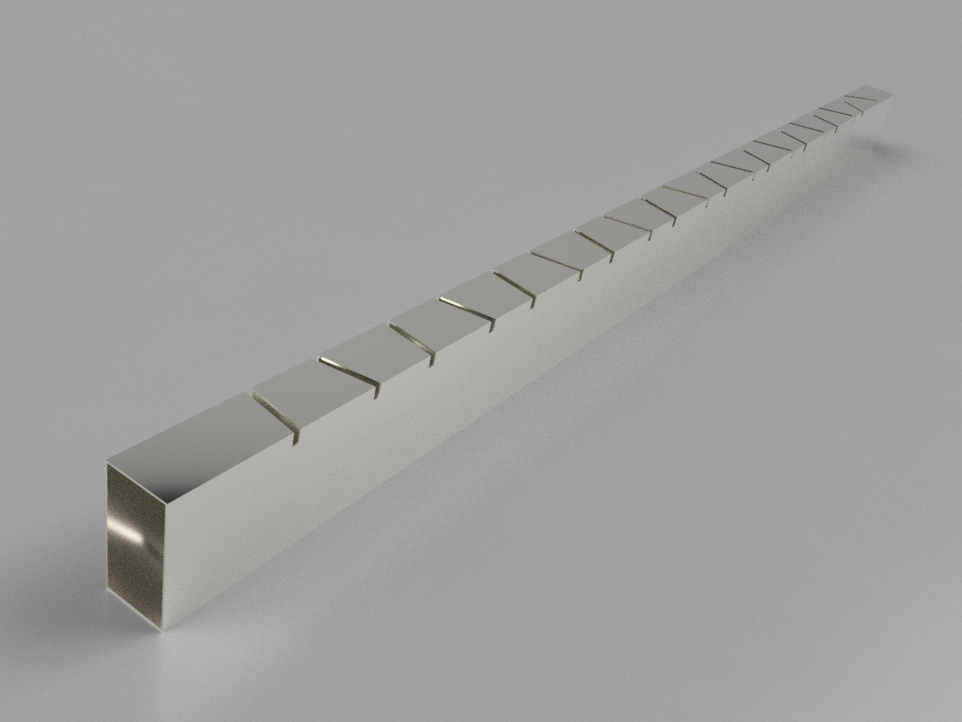
\includegraphics[width=0.95\linewidth,frame]{images/slotted_antenna v1.png}
        \captionof{figure}{\small 3D-Render des Hohlschlitzstrahlers in Fusion360}
        \label{fig:slotted_fusion}
    \end{column}

    % Right Column: Content
    \begin{column}{0.5\textwidth}

       \begin{description}[]
            \item[\textbf{In-line}] Linear angeordnete Schlitze
            \item[\textbf{Resonant}] Betrieb auf Resonanzfrequenz
            \item[\textbf{Waveguide}] Hohlleiterstruktur für die Führung der Wellen
            \item[\textbf{Slot array}] Mehrere Schlitze als Antennen-Array
            \item[\textbf{Narrow-wall slots}] Schlitze in der schmalen Hohlleiterwand
        \end{description}

    \end{column}

\end{columns}
\end{frame}

\section{\thesection. Funktionsweise}
\begin{frame}{\thesection.1 Funktionsweise}
    \begin{figure}
        \centering
        \begin{minipage}[t]{0.49\textwidth}
            \centering
            \includegraphics[width=\linewidth]{images/wandstrom.png}
            \caption{Darstellung der Wandströme einer H$_{10}$–Welle.}
            \footnotetext{\tiny Quelle Abbildung 3: \url{https://www.radartutorial.eu/03.linetheory/Hohlleiter.de.html}}
        \end{minipage}
        \hfill
        \begin{minipage}[t]{0.49\textwidth}
            \centering
            \includegraphics[width=\linewidth]{images/eplanation.png}
            \caption{Unterbrechung von Wandströmen}
        \end{minipage}
        \footnotetext{\tiny Quelle Abbildung 4: Kumar, K. P. Ray: Compact Slot Array Antennas for Wireless Communications, Academic Press, 2019}
    \end{figure}
\end{frame}


\begin{frame}{\thesection.2 Funktionsweise}
  \begin{figure}
    \centering
    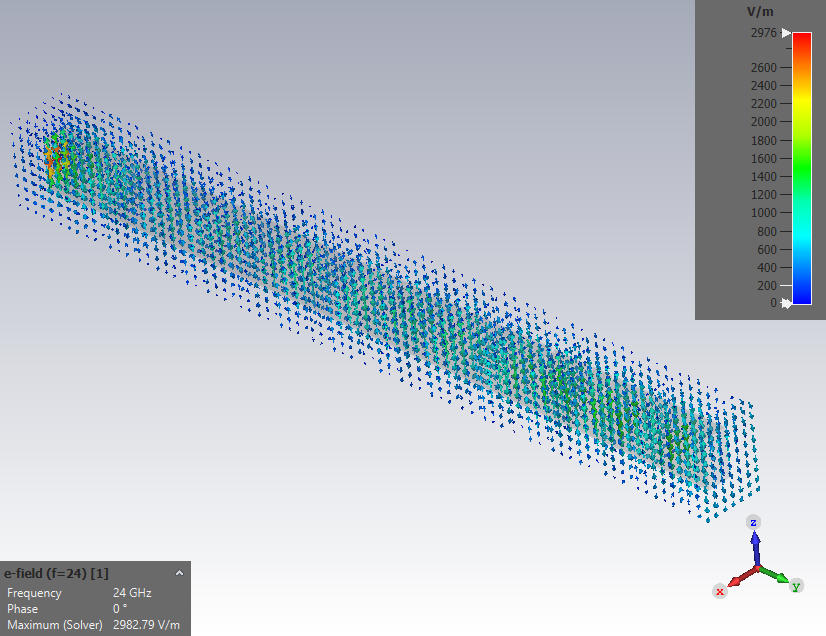
\includegraphics[width=\linewidth]{images/new/e-field (f=24) [1].png}
    \caption{Elektrisches Nahfeld (CST Export)}
  \end{figure}
\end{frame}

\section{\thesection. Nahfeld}
\begin{frame}{\thesection.1 Nahfeld}
    \begin{minipage}[t]{0.48\textwidth}
        \centering
        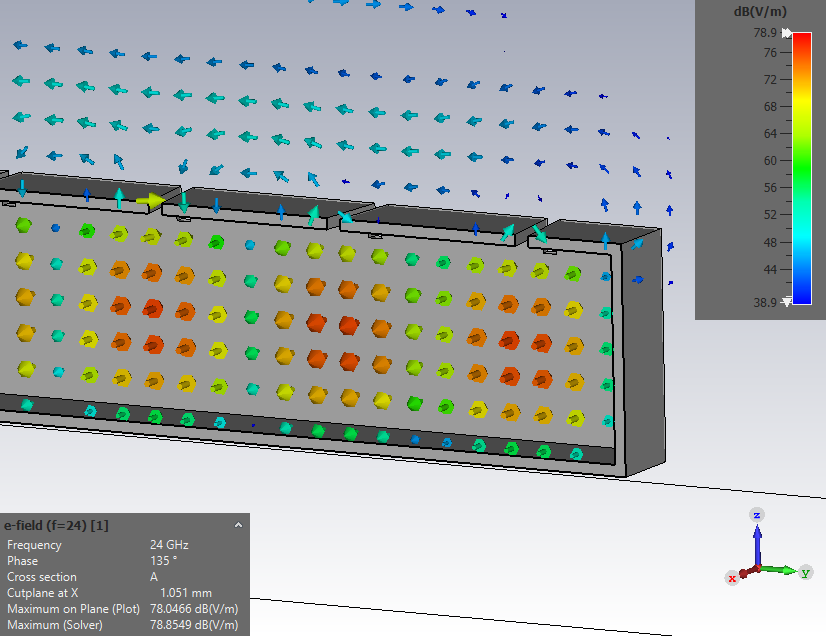
\includegraphics[width=\linewidth]{images/new/e-field (f=24) [1]_2.png}
        \captionof{figure}{Elektrisches Nahfeld (CST Export)}
    \end{minipage}
    \hfill
    \begin{minipage}[t]{0.48\textwidth}
        \centering
        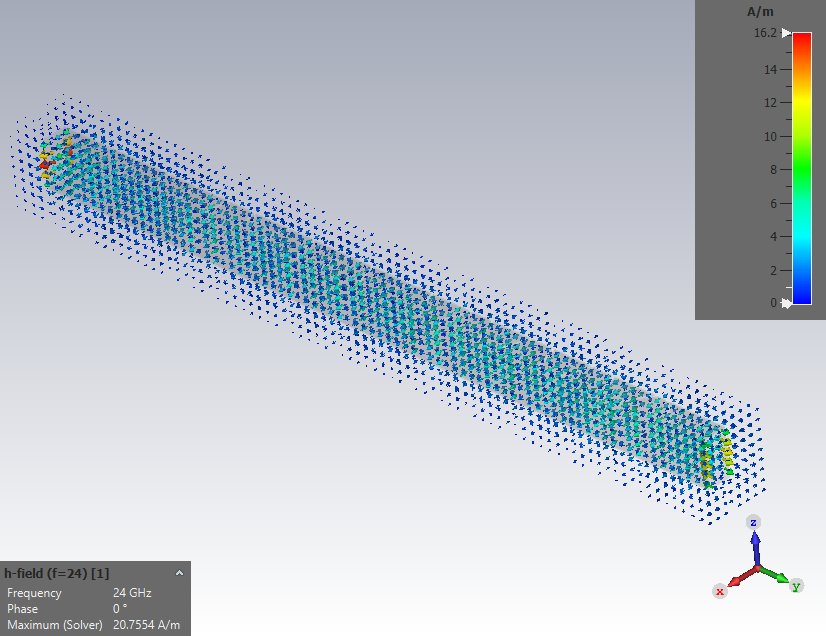
\includegraphics[width=\linewidth]{images/new/h-field (f=24) [1].png}
        \captionof{figure}{Magnetisches Nahfeld (CST Export)}
    \end{minipage}
\end{frame}

\begin{frame}{\thesection.2 Nahfeld}
    \begin{minipage}[t]{0.48\textwidth}
        \centering
        \includegraphics[width=\linewidth]{images/efield_sketch.jpg}
        \captionof{figure}{Elektrisches Nahfeld (CST Export)}
    \end{minipage}
    \hfill
    \begin{minipage}[t]{0.48\textwidth}
        \centering
        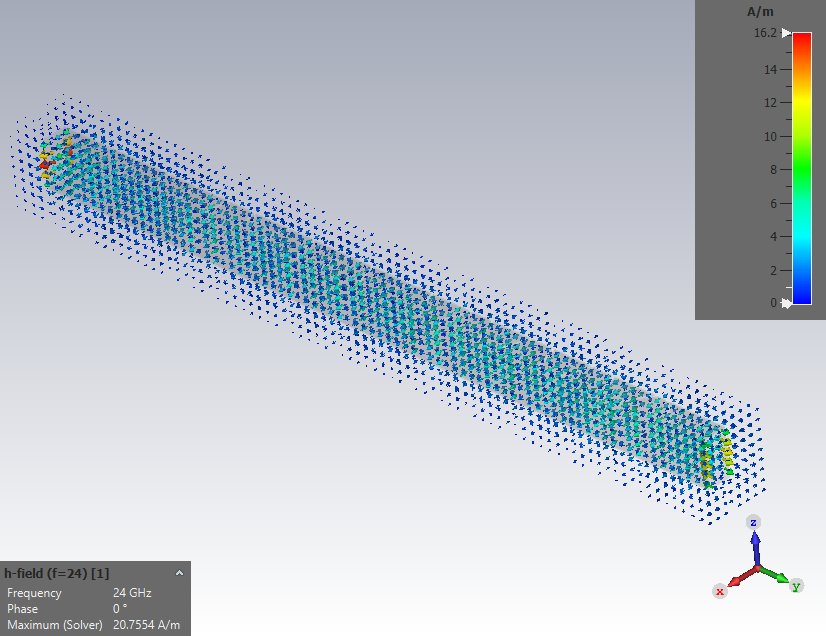
\includegraphics[width=\linewidth]{images/new/h-field (f=24) [1].png}
        \captionof{figure}{Magnetisches Nahfeld (CST Export)}
    \end{minipage}
    \note{
        \begin{minipage}[t]{0.4\textwidth}
            \centering
            \includegraphics[width=\linewidth]{images/eplanation.png}
        \end{minipage}
    }
    \note{\textbf{iplane und hplane cut:}}
\end{frame}

\section{\thesection. Richtwirkung}
\begin{frame}{\thesection. Richtwirkung}
    \centering
    \begin{minipage}[t]{\textwidth}
        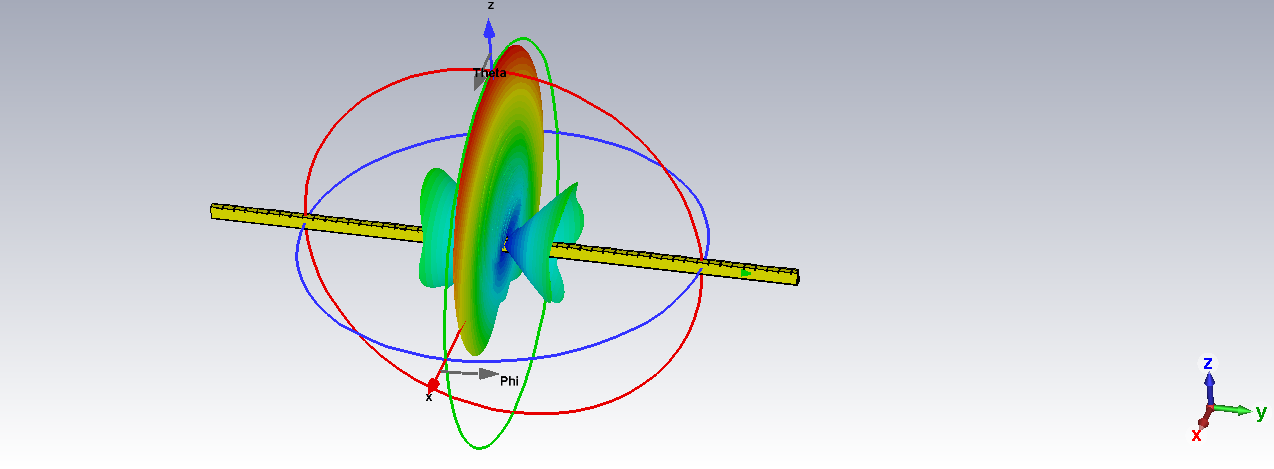
\includegraphics[width=\linewidth]{images/3D_2.png}
        \captionof{figure}{3D-Darstellung der Richtwirkung (CST Render)}
        \label{fig:richtwirkung}
    \end{minipage}
\end{frame}

\section{\thesection. Fernfeld}
\begin{frame}{\thesection. Fernfeld}
    \begin{figure}
        \centering
        \begin{minipage}[t]{0.49\textwidth}
            \centering
            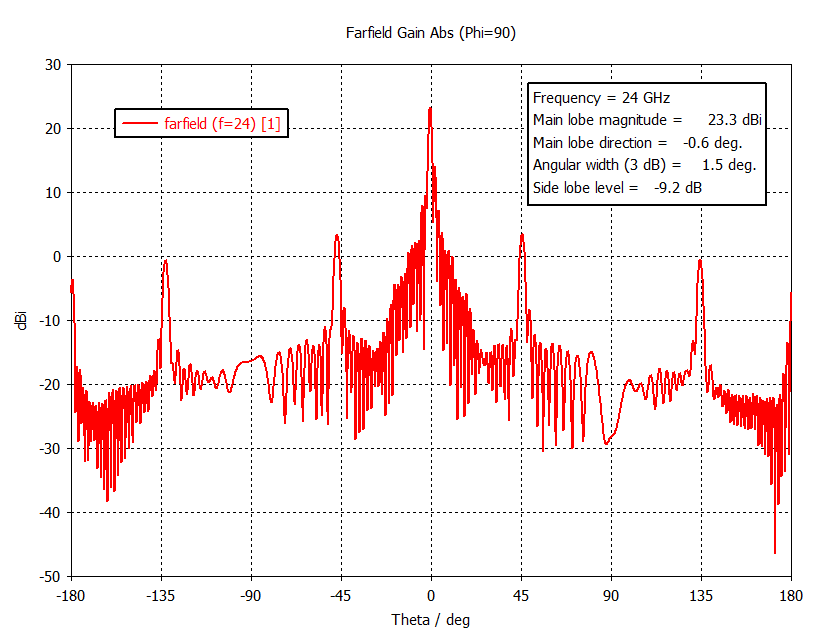
\includegraphics[width=\linewidth]{images/new/90lud.png}
            \caption{Fernfeld h-plane (CST Export)}
        \end{minipage}
        \hfill
        \begin{minipage}[t]{0.49\textwidth}
            \centering
            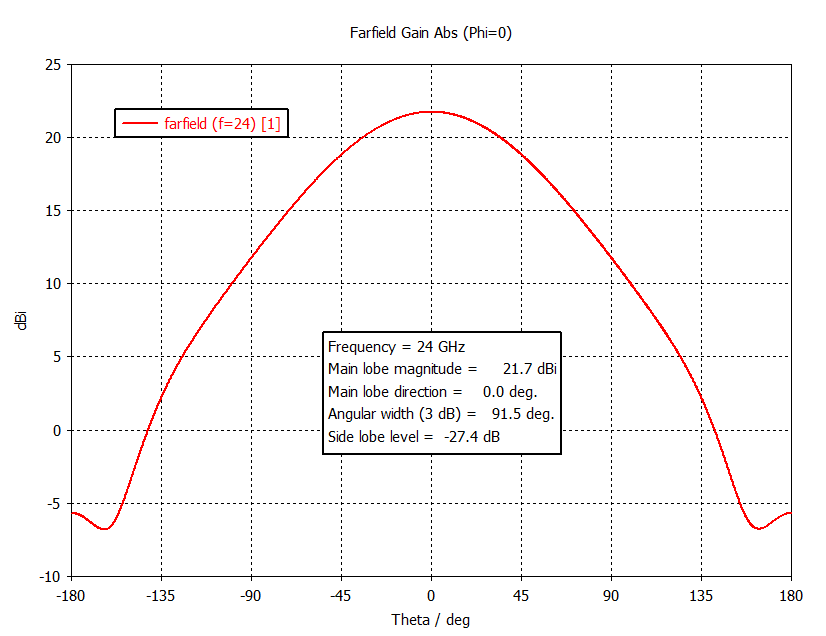
\includegraphics[width=\linewidth]{images/new/0_ludw.png}
            \caption{Fernfeld e-plane (CST Export)}
        \end{minipage}
    \end{figure}
\end{frame}

\section{\thesection. Polarisation}
\begin{frame}{\thesection. Polarisation}
    \begin{figure}
        \centering
        \begin{minipage}[t]{0.49\textwidth}
            \centering
            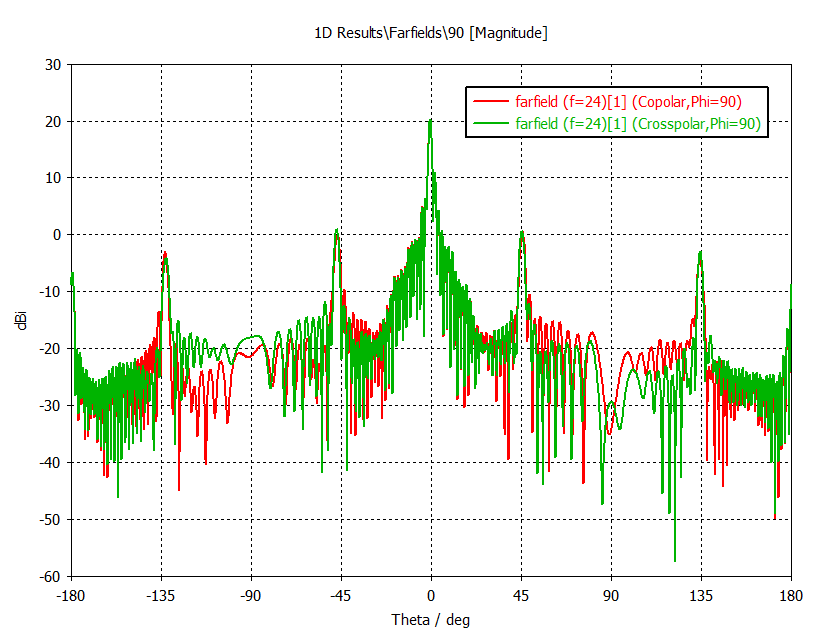
\includegraphics[width=\linewidth]{images/new/90Cro_cros.png}
            \caption{Fernfeld h-plane (CST Export)}
        \end{minipage}
        \hfill
        \begin{minipage}[t]{0.49\textwidth}
            \centering
            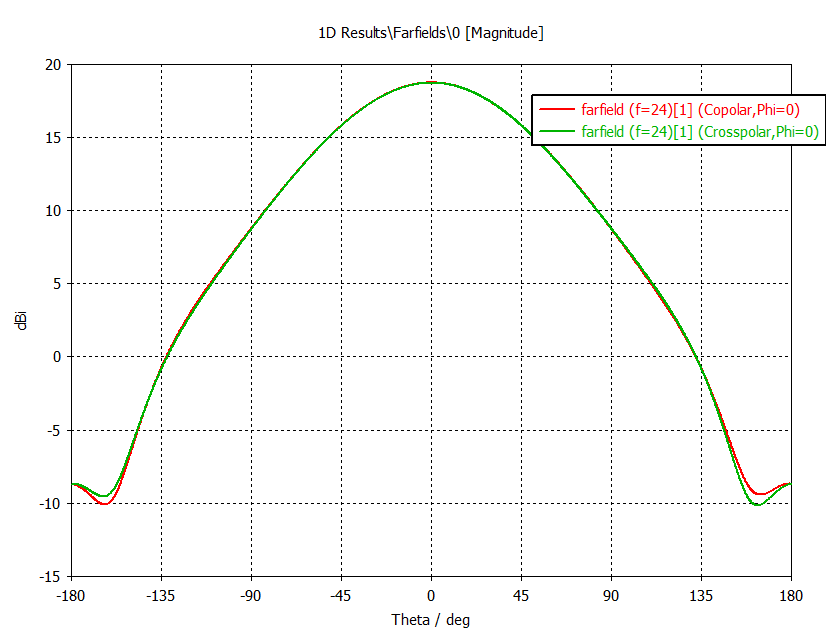
\includegraphics[width=\linewidth]{images/new/0cro_cros.png}
            \caption{Fernfeld e-plane (CST Export)}
        \end{minipage}
    \end{figure}
\end{frame}

\section{\thesection. Streuparameter/Bandbreite}
\begin{frame}{\thesection. Streuparameter/Bandbreite}
    \begin{minipage}[t]{0.48\textwidth}
        \centering
        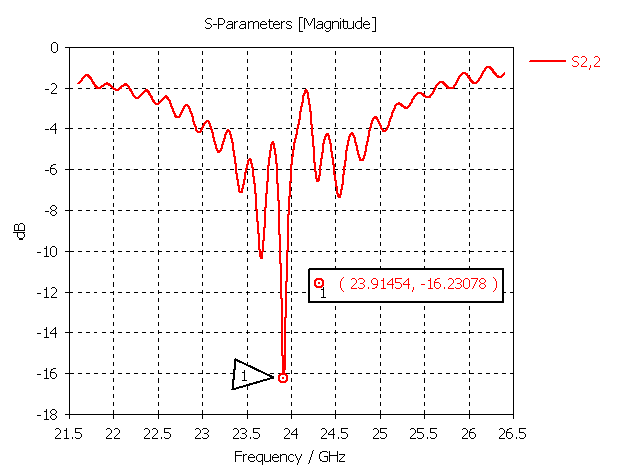
\includegraphics[width=0.9\linewidth]{images/sparamLog.png}
        \captionof{figure}{Reflexionsdämpfung (Logarithmisch)}
    \end{minipage}
    \hfill
    \begin{minipage}[t]{0.48\textwidth}
        \centering
        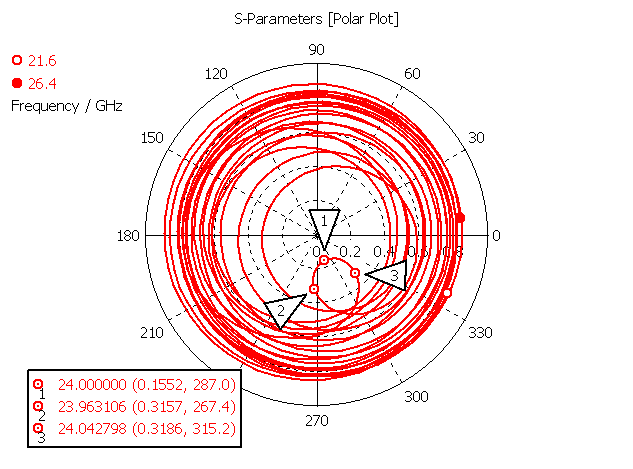
\includegraphics[width=0.9\linewidth]{images/sparamPolar.png}
        \captionof{figure}{Reflexionsdämpfung (Polar)}
    \end{minipage}
\end{frame}

\note{
S₁₁ (Reflexion)
\begin{itemize}
    \item  S₁₁ = 0 dB → 100 Reflexion (schlechtes Matching, z.B. offenes Ende)\\
    \item S₁₁ = –10 dB → ca. 10\% reflektierte Leistung, 90\% werden übertragen\\
    \item S₁₁ = –20 dB → ca. 1\%  Reflexion → sehr gutes Matching\\
    \item S₁₁ = –30 dB → ca. 0,1\%  Reflexion\\
\end{itemize}
}

% \section{\thesection. Gewinn}
% \begin{frame}{\thesection. Gewinn}
% \centering
% \begin{itemize}
%     \item \textbf{Absoluter Gewinn:} \\
%     $G_\text{abs} = 23{,}4\,\mathrm{dBi}$ 
    
%     \note{\textbf{Absoluter Gewinn:} Strahlungsverstärkung der Antenne inklusive interner Verluste (z.\,B. Leitungsverluste, Dielektrika), aber ohne Berücksichtigung des Rückflussverlusts (\gls*{s11}).\\}

%     \item \textbf{Realisierter Gewinn:}
% \end{itemize}

% \begin{align*}
% G_\text{real} &= G \cdot (1 - |S_{11}|) \\
%               &= 23{,}4\,\mathrm{dBi} \cdot (1 - 0{,}158489) \\
%               &\approx 19{,}7\,\mathrm{dBi}
% \end{align*}

% \note{\textbf{Realisierter Gewinn:} Das, was nach allen Verlusten und Rückkopplungen (\gls*{s11}) noch abgestrahlt wird – also der realistischste Wert.\\}
% \end{frame}


\section{\thesection. Berechnungen}
\begin{frame}{\thesection. Berechnungen}
\footnotesize
\begin{tabular}{@{}p{0.15\textwidth}p{0.35\textwidth}p{0.45\textwidth}@{}}
\textbf{Größe} & \textbf{Allgemein} & \textbf{Für meine Schlitzantenne} \\
\midrule
\text{HPBW}_\text{uni} & $\text{HPBW}_\text{uni} \approx \dfrac{50{,}76^\circ}{N \cdot d/\lambda}$ 
& $N = 50$, $d = 8{,}74$mm, $\lambda = 12{,}45$mm \newline
$\Rightarrow \text{HPBW} \approx \mathbf{1{,}4^\circ}$ \\
% \midrule
% Richtwirkung Dipol & $D_\text{hertz} = \dfrac{3}{2} \approx 1{,}76$dBi 
% & Nicht relevant für Gruppenstrahler \\
\midrule
HPBW Dipol & $\text{HPBW}_\text{hertz} = 90^\circ$ 
& Gilt vertikal für jeden Schlitz (dipolähnlich) \\
\midrule
Richtwirkung Gesamt & $\displaystyle D \approx \dfrac{41253}{\Theta_\text{min} \cdot \Theta_\text{max}}$ 
& Mit $\Theta_\text{min} \approx 1{,}4^\circ$, $\Theta_\text{max} \approx 90^\circ$ \newline
$\Rightarrow D \approx \mathbf{327}$ \\
\end{tabular}

\vspace{3mm}
\footnotesize
\textbf{Parameter:} \\
$N$: Anzahl der Strahlerelemente, \quad
$d$: Abstand zwischen den Elementen, \quad
$\lambda$: Wellenlänge, \\
$\text{HPBW}$: Halbwertsbreite der Hauptkeule (3 dB), \quad
$D$: Richtwirkung (Direktivität), \quad
$\Theta_\text{min}, \Theta_\text{max}$: kleinste bzw. größte 3-dB-Keulenbreite (in Grad)
\end{frame}

\section{\thesection. Vergleich: Specs/Calcs/Simul}

\begin{frame}{\thesection. Spezifikationen: Mechanisch}
\begin{columns}[T]
  \begin{column}{0.4\textwidth}
    \begin{minipage}[t]{\linewidth}
         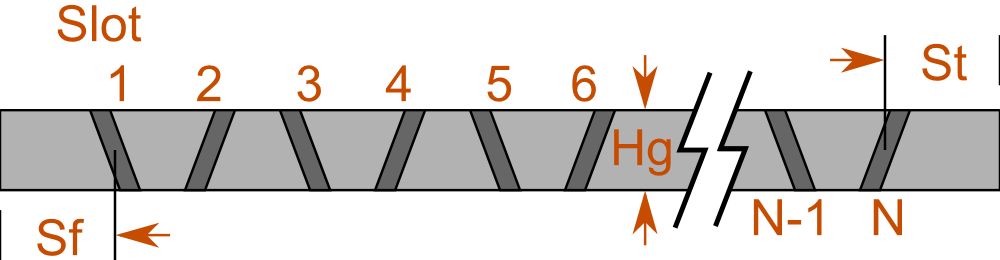
\includegraphics[width=\linewidth]{images/sideviewscets.png}
        \captionof{figure}{Skizze des Hohlleiters aus Antenna Magus}
        \label{fig:magus_sketch}
    \end{minipage}
  \end{column}

  \begin{column}{0.7\textwidth}
    \centering
    \scriptsize
    % \textbf{Mechanische Parameter}
    \vspace{1mm}
    
\begin{table}[h!]
\centering
\caption{Mechanische Parameter}
\begin{tabular}{|l|c|c|c|}
\hline
\textbf{Parameter} & \textbf{Gewünscht} & \textbf{Berechnet} & \textbf{Generiert mit Magus} \\
\hline
Anzahl Slots & – & – & \textbf{50} \\
Slotabstand & – & $\lambda \cdot \tfrac{7}{10}$ & 8{,}74\,mm \\
Slotbreite & – & $\lambda / 20$ & 624{,}6\,\textmu m \\
Slotwinkelbereich & – & - & 5{,}5$^\circ$–8{,}82$^\circ$ \\
Slottiefebereich & – & - & 878{,}26–894{,}46\,\textmu m \\
Wellenleiterbreite & - & - & 8{,}93\,mm \\
Wellenleiterhöhe & - & - & 3{,}97\,mm \\
Wellenleiterlänge & – & – & 44{,}13\,cm \\
Material & Silber & – & Silber \\
\hline
\end{tabular}
\vspace{3mm}
\scriptsize Realisierung durch Einschränkungen von Antenna Magus limitiert
\label{tab:waveguide_summary}
\end{table}
  \end{column}
\end{columns}

\note{\textbf{Slotbreite:}
$\lambda$/20: Schmal genug, um als einfacher Schlitzstrahler zu funktionieren (kein Multimodenverhalten), aber breit genug, um Leistung zu koppeln und mechanisch herstellbar zu sein.\\
Breiter als $\lambda$/10: Mehrere Moden möglich (unerwünscht), mehr Rückreflexion (Impedanzproblem), ungenaue Strahlungsrichtung.\\
Schmaler als $\lambda$/30: Kopplung verschlechtert sich, geringerer Wirkungsgrad, Fertigung wird kritisch.\\}
\end{frame}

\note{
\newpage
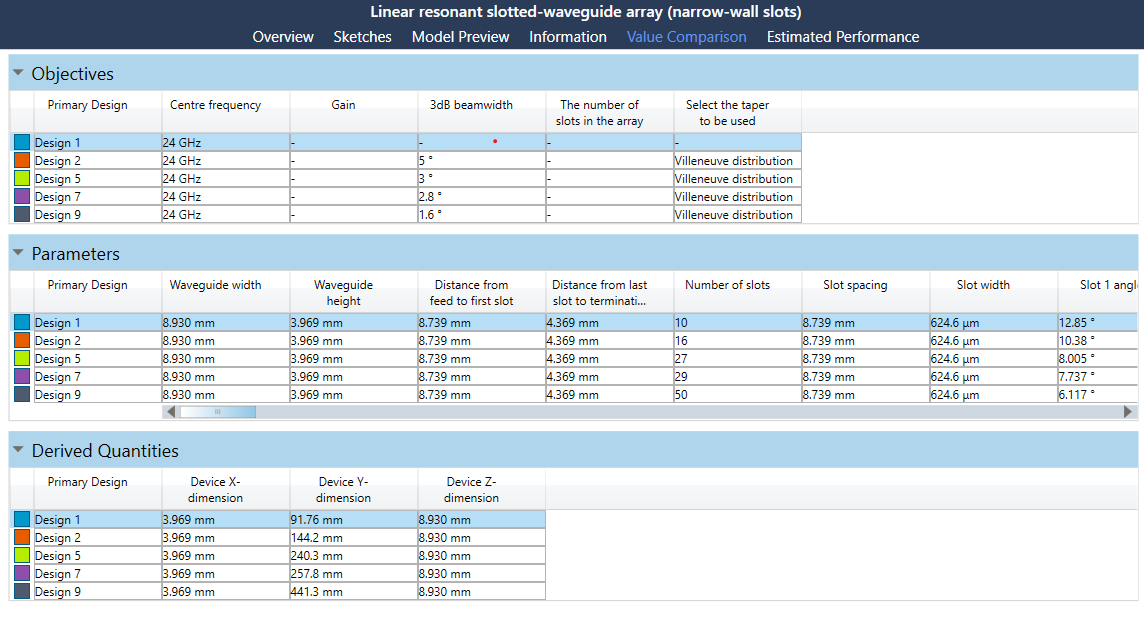
\includegraphics[width=\linewidth]{images/slotNCompariosn.png}
\newpage
\includegraphics[width=0.5\linewidth]{images/reflection_diag.png}
}

\begin{frame}{\thesection. Spezifikationen: Schlitzwinkel und -tiefe}
    \centering
    \begin{minipage}[t]{\textwidth}
        \includegraphics[width=\linewidth]{images/SlotAngleVSNumber.png}
        \captionof{figure}{python plots}
        \label{fig:richtwirkung}
    \end{minipage}
\end{frame}

\begin{frame}{\thesection. Spezifikationen: Elektrisch}
\centering
\footnotesize
\begin{table}[h!]
\caption{Elektrische Parameter}
\label{tab:waveguide_summary}
\begin{tabular}{|l|c|c|c|}
  \hline
  \textbf{Parameter} & \textbf{Gewünscht} & \textbf{Berechnet} & \textbf{Simuliert} \\
  \hline
  Frequenz (Mittenfrequenz) & 24{,}0~GHz & – & 24{,}0~GHz \\
  \hline
  Maximaler Gain & – & – & 23{,}0~dBi (h) \textbar{} 22{,}6~dBi (e) \\
  \hline
  Realisierter Gain & – & – & 22{,}8~dBi (h) \textbar{} 22{,}4~dBi (e) \\
  \hline
  $HPBW_{\mathrm{hplane}}$ & $\leq$ 1{,}0° & 1{,}4° & \textcolor{red}{1{,}6°} \\
  \hline
  $HPBW_{\mathrm{eplane}}$ & – & 90° (Dipol) & 91{,}5° \\
  \hline
  Richtwirkung & – & 327 & 219 \\
  \hline
\end{tabular}
\vspace{3mm}\\
\scriptsize Realisierung durch Einschränkungen von Antenna Magus limitiert
\end{table}
\end{frame}

\note{\textbf{Wellenlänge:} $\lambda$=C/f, hier: 12.49 mm\\
\textbf{Slotabstände:} Gewählt damit die Antenne in Phase abstrahlt\\
\textbf{Anzahl an Slots:} Mehr Slots: Geringere Bandbreite, höherer Gewinn.\\
\textbf{Antennenlänge:} Hat nichts mit Frequenz zu tun, einfach länger mit mehr Slots\\
\textbf{E-Plane:} Quer zur Schlitzrichtung \\
\textbf{H-Plane:} Entlang der Schlitzrichtung\\
}

\section*{\thesection. Anhang}
\begin{frame}{\thesection. Anhang: Abkürzungen}
\scriptsize
\begin{tabular}{|l|l|}
\hline
\textbf{Abkürzung} & \textbf{Bedeutung} \\
\hline
HPBW        & Half Power Beam Width (Halbwertsbreite) \\
dBi         & Dezibel gegenüber Isotropstrahler \\
dB          & Dezibel \\
S11         & Rückflussdämpfung (Reflexionsfaktor) \\
GHz         & Gigahertz \\
mm          & Millimeter \\
µm          & Mikrometer \\
$\lambda$   & Wellenlänge (Wavelength) \\
$f$         & Frequenz \\
E-Feld      & Elektrisches Feld \\
H-Feld      & Magnetisches Feld \\
CST         & Computer Simulation Technology \\
\hline
\end{tabular}
\end{frame}

\begin{frame}[allowframebreaks]{\thesection. Anhang: Literatur}
\begin{thebibliography}{}

\bibitem{strauss}
G. Strauß: \textit{Antennen und Wellen}.\\ Manuskript, Pasing: Hochschule Muenchen, Maerz 2022

\bibitem{compactslot}
Kumar, K. P. Ray: \textit{Compact Slot Array Antennas for Wireless Communications},\\ Academic Press, 2019

\bibitem{Fusion}
Autodesk Fusion 360, Autodesk Inc., www.autodesk.com/products/fusion-360

\bibitem{CST}
CST Studio Suite, Version 2023, Dassault Systèmes, www.3ds.com/products-services/simulia/products/cst-studio-suite

\bibitem{Maggus}
Antenna Magus, Version 2023.2, Dassault Systèmes, www.antennamagus.com

\bibitem{Perotoni2014}
Marcelo B. Perotoni, Rodrigo Enjiu: \textit{Design und Bewertung einer Hohlleiter-Schlitzantenne (Slotted Waveguide Antenna, SWA) mit EM-Simulation},\\ Federal University of ABC, CST – Computer Simulation Technology AG, Oktober 2014.\\
\url{https://www.researchgate.net/publication/283683848_Design_and_Analysis_of_Slotted_Waveguide_Antennas_with_EM_Simulation}

\end{thebibliography}
\end{frame}

% \section*{Abbildungsverzeichnis}
% \begin{frame}{Abbildungsverzeichnis}
% \listoffigures
% \end{frame}

\note{
Feedback zu A\&W:\\
\begin{itemize}
        \item 50 Slots zu große Simulationszeit!!
        \item Variablen bei ihren Formeln beschreiben
        \item Bamdbreite diskutieren bei gegebener HPBW macht keinen Sinn
        \item Früher im Semester mit CST anfangen, vielleicht ein Praktikum mit kleinem Dipol?\\
        Vielleicht sogar PCB antenne? <3\\
        Diesen dann in ihrem Labor vermessen?
        \item Größerer Fokus auf Anwendungen von Antennen
    \end{itemize}
}

\includepdf[pages=-]{Aufgaben_AundW_SS2025_.pdf}
\includepdf[pages=-]{hinweise_zur_praesention_modularbeiten(1).pdf}

\end{document}
